Zeigen Sie mit einer geeigneten Methode, dass das abgebildete Diagramm eine gleichmässig beschleunigte Bewegung darstellt.

\begin{center}
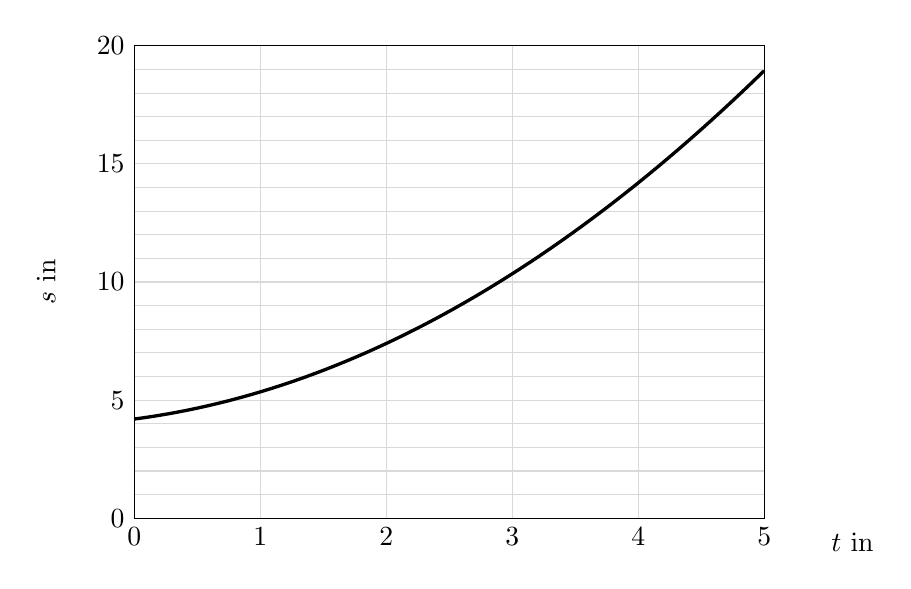
\begin{tikzpicture}[>=stealth, xscale=1.6, yscale=0.3]
 \foreach \x in {1,...,5} \draw[gray!30] (\x,0) -- (\x,20);
 \foreach \y in {1,...,20} \draw[gray!30] (0,\y) -- (5,\y);
 \draw (0,0) rectangle (5,20);
 \foreach \x in {0,...,5} \node[below] at (\x,0) {\x};
 \foreach \y in {0,5,...,20} \node[left] at (0,\y) {\y};
 \node[below] at (5.7,-0.2) {$t$ in \si{\second}};
 \node[rotate=90] at (-0.7,10) {$s$ in \si{\meter}};
 \draw[very thick, domain=0:5, samples=60] plot (\x, {4.2+0.7*\x+0.45*\x*\x});
\end{tikzpicture}
\end{center}
